\documentclass[svgnames]{beamer}
\mode<presentation>
\usefonttheme{serif}
\usecolortheme{dove}
\useinnertheme{rounded}
\setbeamercolor{item projected}{fg=black}
\setbeamertemplate{navigation symbols}{}

\usepackage[english]{babel}
\usepackage[latin1]{inputenc}
\usepackage{times}
\usepackage{amsmath}
\usepackage{amsfonts}
\usepackage{amssymb}
\usepackage{amsthm}
\usepackage{graphics}
\usepackage{multicol}
\usepackage{framed}
\usepackage{ulem}
\usepackage{ifthen}
\usepackage{tikz}
\usepackage{gastex}
\usepackage{ulem}
\usepackage{booktabs}

\newtheorem{conjecture}{Conjecture}

\newcommand{\set}[1]{\{ #1 \}}
\newcommand{\push}{\mathrm{push}}
\newcommand{\pop}{\mathrm{pop}}
\newcommand{\Skip}{\mathrm{skip}}

\newcommand{\parp}{\mathrm{Parity}}
\newcommand{\bound}{\mathrm{Bound}}

\newcommand{\W}{\mathcal{W}}
\newcommand{\WE}{\W_{E}}

\newtheorem{observation}{Observation}
\newtheorem{proposition}{Proposition}

\renewcommand{\ULthickness}{1.2pt}

%%%%%%%%%%%%%%%%%%%%%%%%%%%%%%%%%%%%%%%%%%%%%%%%%%%%%%%%%%%%%%%%%%%%%%%%%%%%%%%
%%%%%%%%%%%%%%%%%%%% A non-original creation by Nathana�l Fijalkow and myself %

\setbeamertemplate{frametitle}{%
  \vskip-2pt%
  \begin{beamercolorbox}[rightskip=2cm,leftskip=1em,dp=1ex,wd=12.8cm]{frametitle}%
    \vskip2pt%
    \usebeamercolor{frametitle}%
    \begin{tikzpicture}[scale=1]%
      \useasboundingbox (0,0) rectangle (0,0); %(-1,-1) rectangle (1,1);%
      \ifthenelse{\insertframenumber<\inserttotalframenumber}%
      { % uncomplete tart

        \pgfmathsetmacro{\aimangle}{90-(\insertframenumber*360/\inserttotalframenumber)}
        \fill [fill=frametitle.fg,thin, color=gray!50,draw=black] (11.8,.2) -- (11.8,.6) arc (90:\aimangle:0.4) -- cycle;%

      }{ % the full tart
        \fill[fill=frametitle.fg,thin, color=gray!50,draw=black] (11.8,0.2) circle (.4);%
      }%
      \fill[fill=frametitle.fg,thin, color=white,draw=black] (11.8,0.2) circle (.3);%
      \node at (11.8, .2) [black,circle]{\normalsize\insertframenumber};

    \end{tikzpicture}
    \insertframetitle%
    \vskip2pt%
  \end{beamercolorbox}%
}
%%%%%%%%%%%%%%%%%%%%%%%%%%%%%%%%%%%%%%%%%%%%%%%%%%%%%%%%%%%%%%%%%%%%%%%%%%%%%%%


\setbeamertemplate{blocks}[rounded]%
\setbeamercolor{block title}{bg=normal text.bg!90!black}
\setbeamercolor{block body}{bg=normal text.bg!95!black}

\AtBeginSection[]
{
\addtocounter{framenumber}{-1}
  \begin{frame}<beamer>{Outline}
    \tableofcontents[currentsection]
  \end{frame}
}

\AtBeginSubsection[]
{
\addtocounter{framenumber}{-1}
  \begin{frame}<beamer>{Outline}
    \tableofcontents[currentsection,currentsubsection]
  \end{frame}
}

\begin{document}

\addtocounter{framenumber}{-1}

\title{Boundedness Games}
\subtitle{S\'eminaire de l'\'equipe MoVe, LIF,\\
Marseille, May 2nd, 2013}
\author{Nathana\"el Fijalkow}
\institute{Institute of Informatics, Warsaw University -- Poland 
\and LIAFA, Universit\'e Paris 7 Denis Diderot -- France}
\date{
\begin{small}
(based on joint works with Krishnendu Chatterjee, Thomas Colcombet, Florian Horn and Martin Zimmermann)
\end{small}}

\begin{frame}
\maketitle
\end{frame}

\begin{frame}{Definition of $\omega B$-games}
\begin{center}
Two-player turn-based games over \textbf{finite} or \textbf{infinite} graphs
\begin{multicols}{2}
\begin{picture}(40,60)(0,0)
	\gasset{Nw=8,Nh=8}
	
  	\rpnode[polyangle=45](1)(30,15)(4,5){}
  	\node(2)(20,30){}
  	\node(3)(40,30){}
  	\rpnode[Nmarks=i,iangle=180,polyangle=45](4)(0,30)(4,5){}
  	\rpnode[polyangle=45](5)(10,50)(4,5){}
  	\node(6)(10,10){}
  	\rpnode[polyangle=45](7)(30,50)(4,5){}

  	\drawedge(1,2){}
  	\drawedge[curvedepth=3](1,3){}
	\drawloop[loopangle=90](2){}
  	\drawedge(2,3){}
  	\drawedge(2,6){}
  	\drawedge[curvedepth=5](3,1){}
  	\drawedge(4,2){}
  	\drawedge[curvedepth=5](4,5){}
  	\drawedge[curvedepth=5](5,4){}
	\drawloop[loopangle=-90](6){}
  	\drawedge(7,5){}

\only<8,15>{
  	\rpnode[polyangle=45](1b)(30,15)(4,5){{\color{red}{$1$}}}
  	\node(2b)(20,30){{\color{blue}{$2$}}}
  	\node(3b)(40,30){{\color{red}{$3$}}}
  	\rpnode[Nmarks=i,iangle=180,polyangle=45](4b)(0,30)(4,5){{\color{red}{$3$}}}
  	\rpnode[polyangle=45](5b)(10,50)(4,5){{\color{blue}{$2$}}}
  	\node(6b)(10,10){{\color{blue}{$4$}}}
  	\rpnode[polyangle=45](7b)(30,50)(4,5){{\color{blue}{$0$}}}
}

\only<9,10,11,12,13,14,15>{
  	\drawedge(1,2){$i,\varepsilon$}
  	\drawedge[curvedepth=3](1,3){$\varepsilon,i$}
	\drawloop[loopangle=90](2){$i,i$}
  	\drawedge(2,3){$\varepsilon,\varepsilon$}
  	\drawedge[ELside=r](2,6){$i,r$}
  	\drawedge[curvedepth=5](3,1){$r,i$}
  	\drawedge(4,2){$\varepsilon,i$}
  	\drawedge[curvedepth=5](4,5){$\varepsilon,i$}
  	\drawedge[ELside=r,curvedepth=5](5,4){$i,i$}
	\drawloop[loopangle=-90](6){$\varepsilon,r$}
  	\drawedge[ELside=r](7,5){$i,\varepsilon$}
	}

\only<3,10>{\drawedge[AHLength=3,AHlength=4,linecolor=red,linewidth=0.7](4,2){}}
\only<5,12>{\drawedge[AHLength=3,AHlength=4,linecolor=red,linewidth=0.7](2,6){}}

\only<2,3,9,10>{\node[fillcolor=magenta,Nw=4,Nh=4](pebble)(0,30){}} 
\only<4,5,11,12>{\node[fillcolor=magenta,Nw=4,Nh=4](pebble)(20,30){}} 
\only<6,13>{\node[fillcolor=magenta,Nw=4,Nh=4](pebble)(10,10){}} 

\end{picture}
\begin{picture}(40,60)(0,0)
	\gasset{Nw=8,Nh=8}
	
\only<1,2,3,4,5,6>{
  	\node(Eve)(10,35){}
	\put(16,34){controlled by Eve}
  	\rpnode[polyangle=45](Adam)(10,25)(4,5){}
	\put(16,24){controlled by Adam}
	}

\only<8>{
	\begin{huge}
	\put(2,40){parity condition:}
	\put(-4,26){the minimal priority}
	\put(-4,18){seen infinitely often}
	\put(8,10){is even}
	\end{huge}
	}	

\only<9,10,11,12,13,14>{
	\begin{huge}
	\put(6,25){$\varepsilon: \textrm{nothing}$}
	\put(6,15){$i: \textrm{increment}$}
	\put(6,5){$r: \textrm{reset}$}
	\end{huge}
	}

\only<9,10>{
	\begin{huge}
	\put(10,50){$c_1 = 0$}
	\put(10,40){$c_2 = 0$}
	\end{huge}
}

\only<11,12>{
	\begin{huge}
	\put(10,50){$c_1 = 0$}
	\put(10,40){$c_2 = 1$}
	\end{huge}
}

\only<13,14>{
	\begin{huge}
	\put(10,50){$c_1 = 1$}
	\put(10,40){$c_2 = 0$}
	\end{huge}
}

\only<7,15>{
	\begin{huge}
	\put(-12,50){$\omega B$ winning condition:}
	\put(12,36){parity}
	\put(15,28){and}
	\put(4,20){all counters}
	\put(3,12){are bounded}
	\end{huge}
}

\end{picture}
\end{multicols}
\end{center}
\end{frame}

\begin{frame}{Strategy (for Eve)}
General form 
$$\sigma : V^+ \rightarrow V$$
\pause

Positional or memoryless
$$\sigma : V \rightarrow V$$
\pause
\begin{theorem}[M\"uller and Schupp]
In parity games, both players have memoryless winning strategies.
\end{theorem}
\pause

What about $\omega B$ games?
\pause

\vskip1em
Finite-memory 
$$\left \{
\begin{array}{c}
\sigma : V \times M \rightarrow V \\
\mu : M \times E \rightarrow M
\end{array}
\right.$$
\end{frame}

\begin{frame}{Why finite-memory strategies?}
Thomas Colcombet's habilitation:
\vskip1em

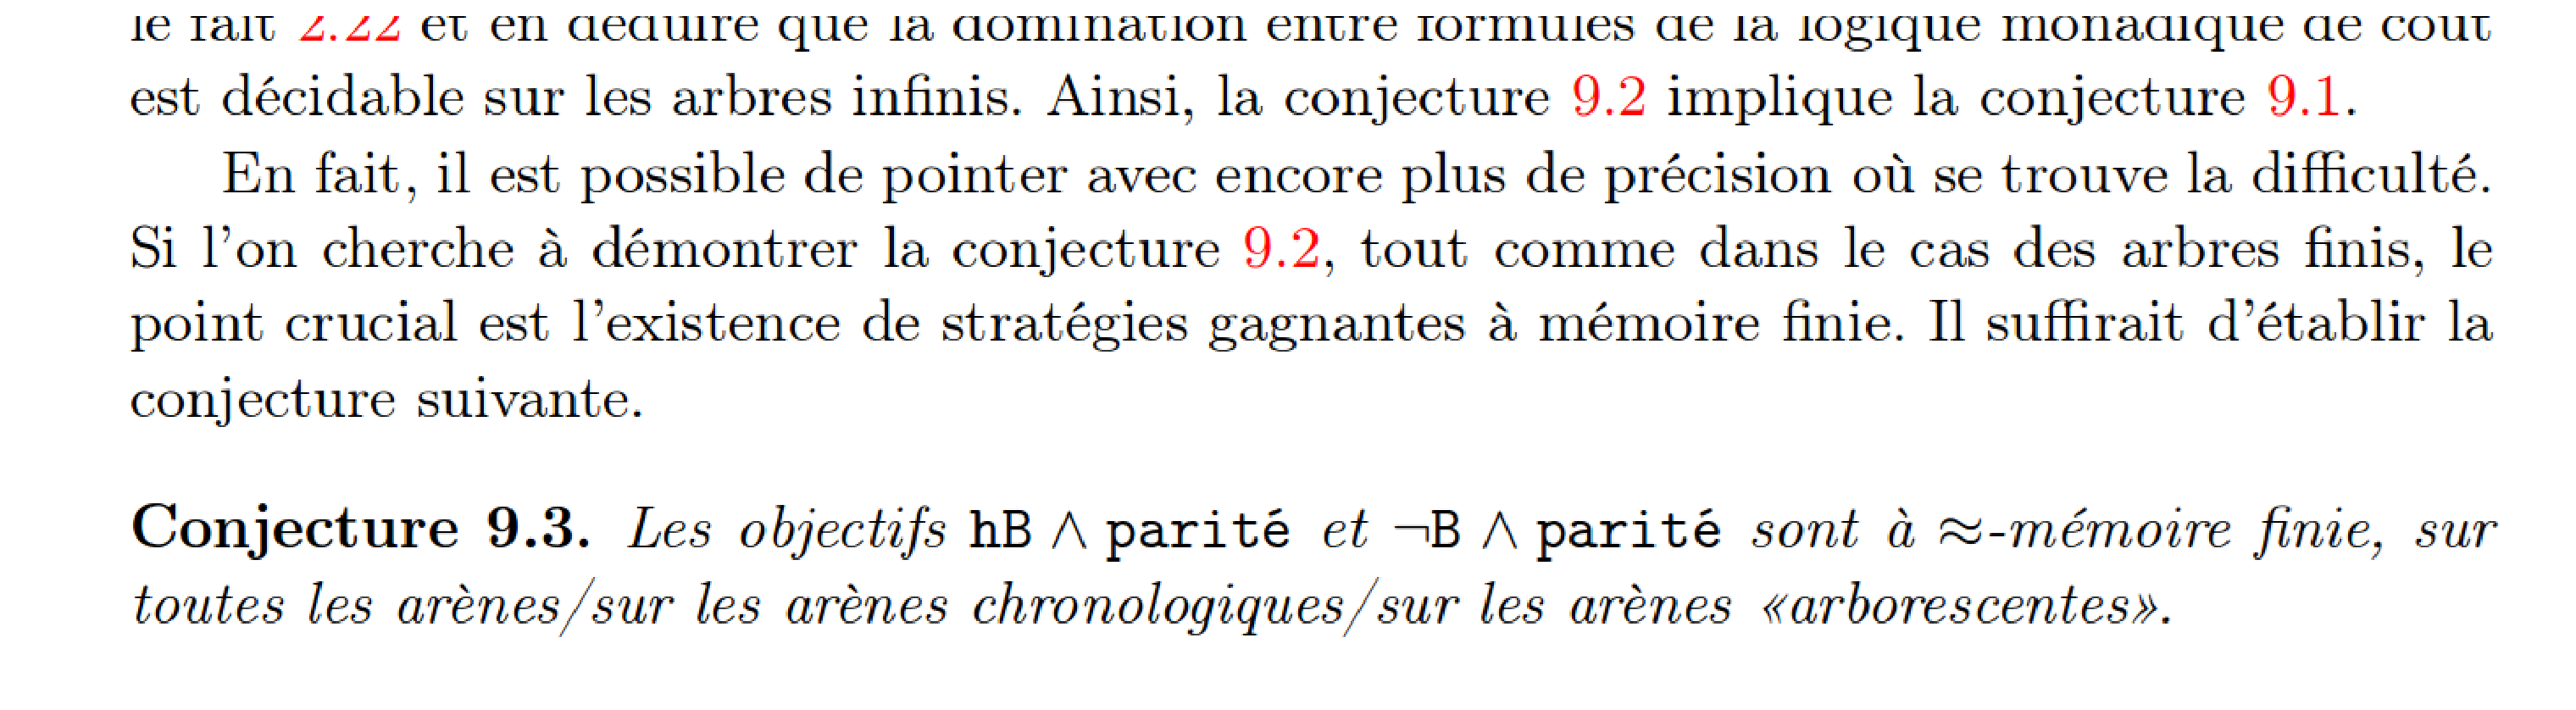
\includegraphics[width=100mm]{thomas_habilitation}

Existence of finite-memory strategies in (some) boundedness games

$\Longrightarrow$ Decidability of cost MSO over infinite trees

$\Longrightarrow$ Decidability of the index of the non-deterministic Mostowski's hierarchy
(open for 40 years)!
\end{frame}

\begin{frame}{Quantification}
Eve wins means:

\begin{figure}[ht]
\begin{minipage}[b]{0.45\linewidth}
\centering
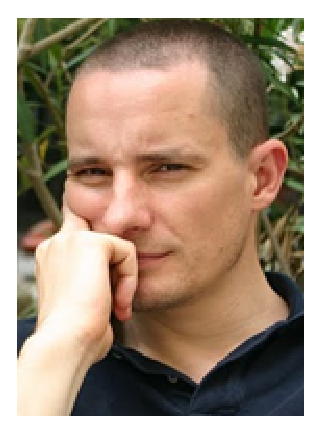
\includegraphics[width=19mm]{mikolaj}

$\exists \sigma$ (strategy for Eve),

$\forall \pi$ (paths), 

$\exists N \in \mathbb{N}$,

\end{minipage}
\hspace{0.5cm}
\begin{minipage}[b]{0.45\linewidth}
\centering
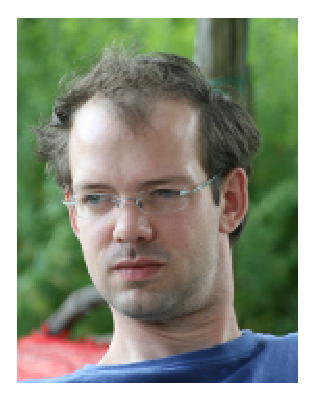
\includegraphics[width=20mm]{thomas}

$\exists \sigma$ (strategy for Eve),

$\exists N \in \mathbb{N}$,

$\forall \pi$ (paths),
\end{minipage}
\end{figure}
\begin{center}
$\pi$ satisfies parity
and each counter is bounded by $N$.
\end{center}

\pause
Is this:
\begin{enumerate}
	\item Equivalent? \only<3>{\textcolor{red}{Sometimes \ldots}}
	\item Decidable? \only<3>{\textcolor{red}{Not always \ldots}}
\end{enumerate}
\end{frame}


\begin{frame}{The questions I am interested in}
Boundedness games:
\begin{enumerate}
	\item Over finite graphs: decide the winner
	\textcolor{red}{efficiently} and construct \textcolor{red}{small} finite-memory strategies.
	\pause
	
	$\looparrowright$ Cost-parity games~[F. and Zimmermann, 2012].
	\pause
	\item Over pushdown graphs: decide the winner
	and construct finite-memory strategies.
	\pause
	
	$\looparrowright$ Pushdown $\omega B$ games~[Chatterjee and F., 2013].
	\pause
	\item Over infinite graphs: prove the existence
	of finite-memory winning strategies.
	\pause
	
	$\looparrowright$ Ongoing work with Thomas Colcombet and Florian Horn.
\end{enumerate}
\end{frame}

\begin{frame}{Outline}
    \tableofcontents
\end{frame}

\section{Finite-memory strategies}

\subsection{Some examples}

\begin{frame}{Eve needs some memory}
\begin{figure}
\begin{center}
\begin{picture}(45,40)(0,0)
	\gasset{Nw=7,Nh=7}

  	\rpnode[polyangle=45,Nmarks=i](0)(0,20)(4,5){$v_0$}
	\imark[iangle=200](0)
	\imark[iangle=160](0)

  	\node(12)(20,40){$v_{1,2}$}
  	\node(13)(20,20){$v_{1,3}$}
  	\node(23)(20,0){$v_{2,3}$}

  	\drawedge(0,12){}
  	\drawedge(0,13){}
  	\drawedge(0,23){}

  	\node[linecolor=White](invisible12)(45,40){\large{\ to $v_0$}}
  	\node[linecolor=White](invisible13)(45,20){\large{\ to $v_0$}}
  	\node[linecolor=White](invisible23)(45,0){\large{\ to $v_0$}}

  	\drawedge[curvedepth=5](12,invisible12){$i_1,r_2$}
  	\drawedge[curvedepth=-5](12,invisible12){$r_1,i_2$}

  	\drawedge[curvedepth=5](13,invisible13){$i_1,r_3$}
  	\drawedge[curvedepth=-5](13,invisible13){$r_1,i_3$}

  	\drawedge[curvedepth=5](23,invisible23){$i_2,r_3$}
  	\drawedge[curvedepth=-5](23,invisible23){$r_2,i_3$}
\end{picture}
\end{center}
\end{figure}
\end{frame}

\begin{frame}{Adam needs infinite memory}
\begin{figure}
\begin{center}
\begin{picture}(100,25)(0,0)
	\rpnode[Nmarks=i,polyangle=45](v_0)(0,10)(4,4){}

	\rpnode[polyangle=45](v_1)(12,20)(4,4){}
	\rpnode[polyangle=45](v_2)(24,20)(4,4){}
	\rpnode[polyangle=45](v_3)(36,20)(4,4){}
	\put(41,20){\begin{large}$\ldots$\end{large}}

	\rpnode[polyangle=45](u_1)(12,0)(4,4){}
	\rpnode[polyangle=45](u_2)(24,0)(4,4){}
	\rpnode[polyangle=45](u_3)(36,0)(4,4){}
	\put(41,0){\begin{large}$\ldots$\end{large}}

	\drawedge(v_0,v_1){}
	\drawedge(u_1,v_0){$r$}
	\drawedge(v_1,v_2){}
	\drawedge(u_2,u_1){$i$}
	\drawedge(v_1,u_1){}
	\drawedge(v_2,u_2){}
	\drawedge(v_2,v_3){}
	\drawedge(u_3,u_2){$i$}
	\drawedge(v_3,u_3){}

\only<2>{
	\rpnode[Nmarks=i,polyangle=45](push)(70,8)(4,4){}
	\rpnode[polyangle=45](pop)(85,8)(4,4){}

	\drawedge[curvedepth=2](push,pop){}
	\drawedge[curvedepth=2](pop,push){$\begin{array}{c} \bot \\ r \end{array}$}
	\drawloop[loopdiam=8,loopangle=90](push){$\begin{array}{c} \push(a) \\ \varepsilon \end{array}$}
	\drawloop[loopdiam=8,loopangle=90](pop){$\begin{array}{c} \pop(a) \\ i \end{array}$}
}
\end{picture}
\end{center}
\end{figure}
\end{frame}

\begin{frame}{Eve needs infinite memory}
\begin{figure}
\begin{center}
\begin{picture}(40,60)(0,0)
	\gasset{Nh=5,Nw=5}

	\rpnode[polyangle=45](u_0)(0,0)(4,4){$0$}
	\rpnode[polyangle=45](u_1)(0,15)(4,4){$0$}
	\rpnode[polyangle=45](u_2)(0,30)(4,4){$0$}
	\rpnode[Nmarks=i,polyangle=45](u_3)(0,45)(4,4){$0$}

	\node(v_0)(20,0){$1$}
	\node(v_1)(20,15){$1$}
	\node(v_2)(20,30){$1$}
	\node(v_3)(20,45){$1$}

	\drawedge(u_0,v_0){}
	\drawedge(u_1,u_0){}
	\drawedge(u_1,v_1){}
	\drawedge(u_2,u_1){}
	\drawedge(u_2,v_2){}
	\drawedge(u_3,u_2){}
	\drawedge(u_3,v_3){}

	\node(fini)(30,60){$0$}
	\drawedge(v_3,fini){$i$}
	\drawloop[loopangle=45](fini){}

\only<1,2>{
	\drawedge[curvedepth=-3,ELside=r](v_0,v_1){$i$}
	\drawedge[curvedepth=-3,ELside=r](v_1,v_2){$i$}
	\drawedge[curvedepth=-3,ELside=r](v_2,v_3){$i$}
}

\only<2>{
	\node[fillcolor=red](v_0)(20,0){$1$}
	\node[fillcolor=blue](v_1)(20,15){$1$}
	\node[fillcolor=red](v_2)(20,30){$1$}
	\node[fillcolor=blue](v_3)(20,45){$1$}

}
	\drawedge[curvedepth=-3,ELside=r](v_1,v_0){$r$}
	\drawedge[curvedepth=-3,ELside=r](v_2,v_1){$r$}
	\drawedge[curvedepth=-3,ELside=r](v_3,v_2){$r$}

\only<3>{
	\rpnode[polyangle=45](w_0)(40,0)(4,4){$1$}
	\rpnode[polyangle=45](w_1)(40,15)(4,4){$1$}
	\rpnode[polyangle=45](w_2)(40,30)(4,4){$1$}
	\rpnode[polyangle=45](w_3)(40,45)(4,4){$1$}

	\drawedge(v_0,w_1){$i$}
	\drawedge(v_1,w_2){$i$}
	\drawedge(v_2,w_3){$i$}

	\drawedge(w_0,v_0){}
	\drawedge(w_0,w_1){}
	\drawedge(w_1,v_1){}
	\drawedge(w_1,w_2){}
	\drawedge(w_2,v_2){}
	\drawedge(w_2,w_3){}
	\drawedge(w_3,v_3){}

	\node[Nframe=n](i_0)(50,0){}
	\node[Nframe=n](i_1)(50,15){}
	\node[Nframe=n](i_2)(50,30){}
	\node[Nframe=n](i_3)(50,45){}

	\drawedge(w_0,i_0){}
	\drawedge(w_1,i_1){}
	\drawedge(w_2,i_2){}
	\drawedge(w_3,i_3){}
}
\end{picture}
\end{center}
\end{figure}
\end{frame}

\begin{frame}{Conjecture's status}

\begin{conjecture}[Thomas Colcombet's conjecture]
Over arbitrary graphs / chronological graphs / tree-like graphs,\\
\begin{center}
if Eve has a strategy ensuring $\parp \cap \bound(N)$,\\
then she has a finite-memory strategy (of size independent of $N$)
ensuring $\parp \cap \bound(\alpha(N))$.
\end{center}
\end{conjecture}
\pause

\begin{theorem}
The conjecture does not hold over arbitrary graphs.
\end{theorem}

\pause

With some more effort:

\begin{theorem}
The conjecture does not hold over chronological graphs.
\end{theorem}
\end{frame}

\begin{frame}{Potato-trees}
\begin{figure}
\begin{center}
\begin{picture}(90,60)(0,0)
	\gasset{Nw=7,Nh=7}

  	\node[linecolor=White](rootR)(47,58){}
  	\node[linecolor=White](0R)(17,28){}
  	\node[linecolor=White](1R)(77,28){}
  	\node[linecolor=White](00R)(2,-2){}
  	\node[linecolor=White](01R)(32,-2){}
  	\node[linecolor=White](10R)(62,-2){}
  	\node[linecolor=White](11R)(92,-2){}

  	\node[linecolor=White](rootL)(41,59){}
  	\node[linecolor=White](0L)(11,29){}
  	\node[linecolor=White](1L)(71,29){}
  	\node[linecolor=White](00L)(-4,-1){}
  	\node[linecolor=White](01L)(26,-1){}
  	\node[linecolor=White](10L)(56,-1){}
  	\node[linecolor=White](11L)(86,-1){}

  	\node[linecolor=White](root)(45,60){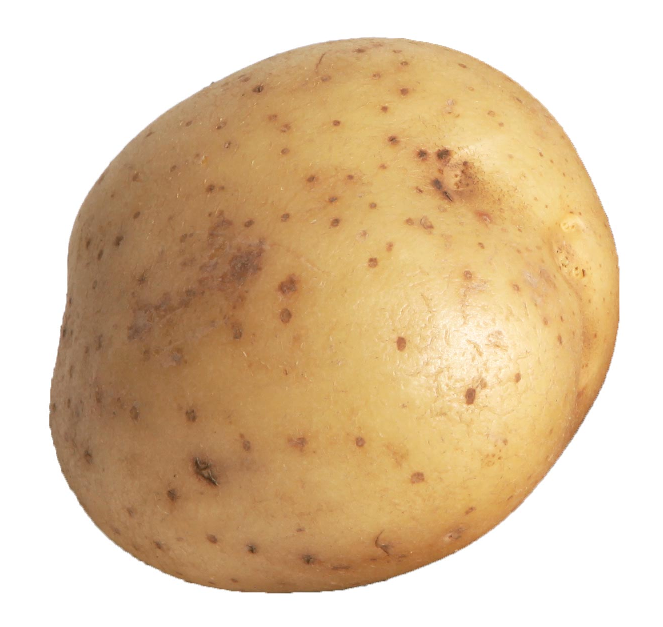
\includegraphics[width=15mm]{potato}}
  	\node[linecolor=White](0)(15,30){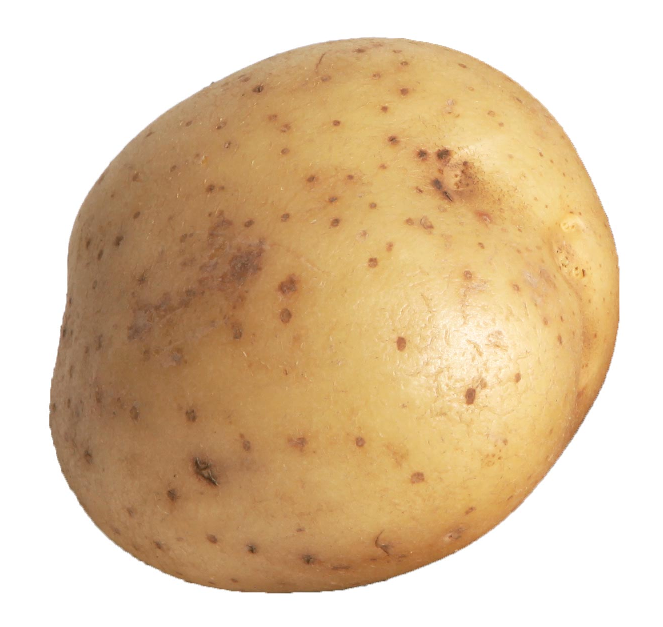
\includegraphics[width=15mm]{potato}}
  	\node[linecolor=White](1)(75,30){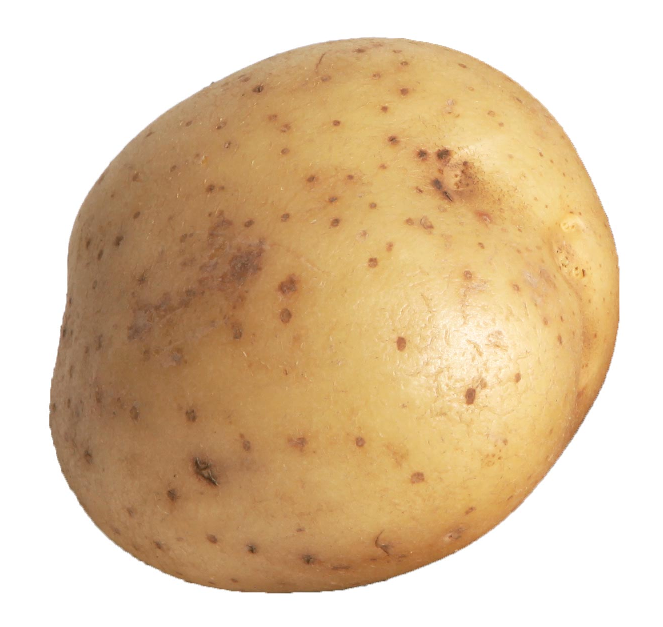
\includegraphics[width=15mm]{potato}}
  	\node[linecolor=White](00)(0,0){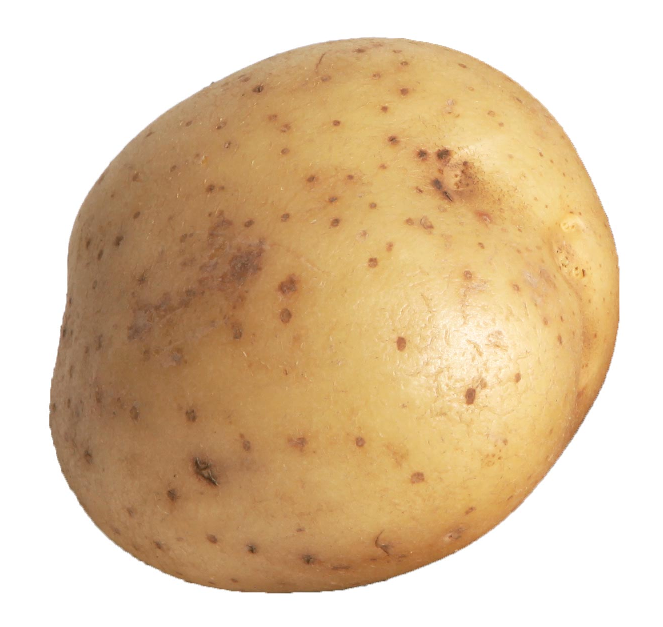
\includegraphics[width=15mm]{potato}}
  	\node[linecolor=White](01)(30,0){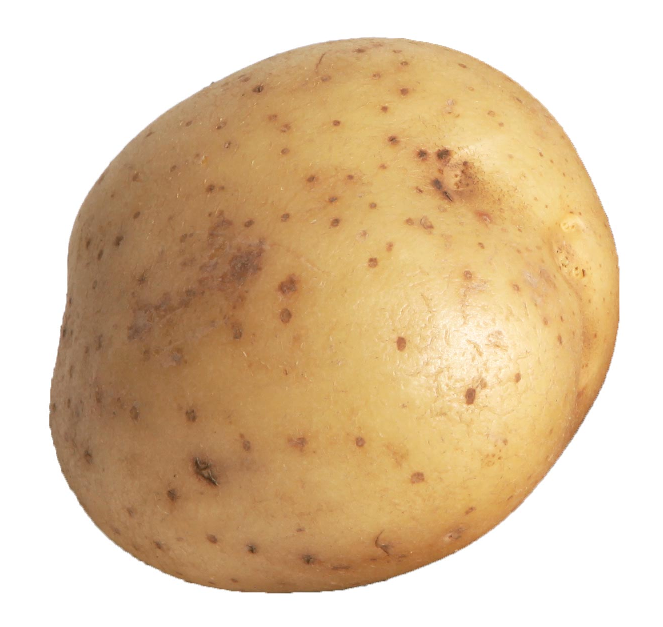
\includegraphics[width=15mm]{potato}}
  	\node[linecolor=White](10)(60,0){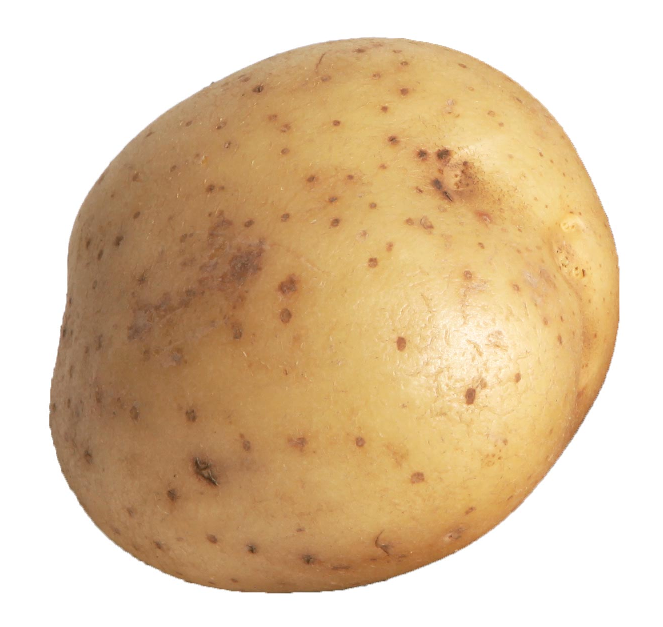
\includegraphics[width=15mm]{potato}}
  	\node[linecolor=White](11)(90,0){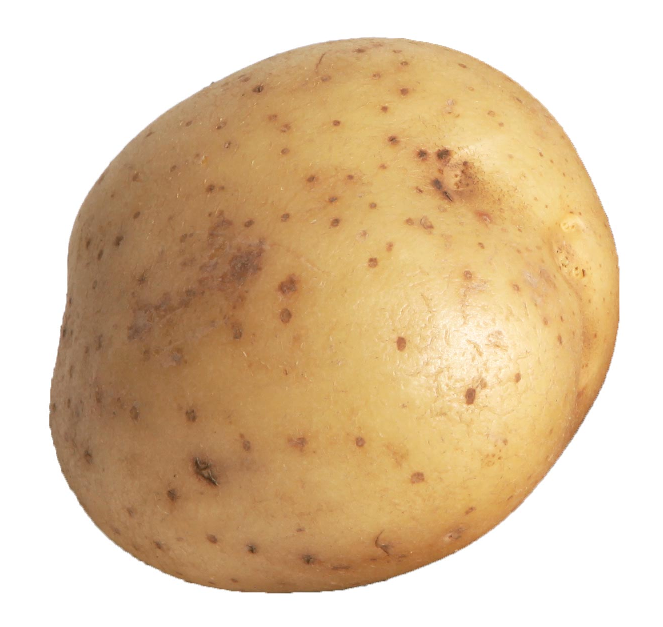
\includegraphics[width=15mm]{potato}}

  	\drawedge(root,0){}
  	\drawedge(root,1R){}
  	\drawedge(0,00L){}
  	\drawedge(0,01){}
  	\drawedge(1,10R){}
  	\drawedge(1,11L){}

  	\drawedge(rootR,0R){}
  	\drawedge(rootR,1L){}
  	\drawedge(0R,00){}
  	\drawedge(0R,01R){}
  	\drawedge(1R,10L){}
  	\drawedge(1R,11){}

  	\drawedge(rootL,0L){}
  	\drawedge(rootL,1){}
  	\drawedge(0L,00R){}
  	\drawedge(0L,01L){}
  	\drawedge(1L,10){}
  	\drawedge(1L,11R){}
\end{picture}
\end{center}
\end{figure}
\end{frame}

\subsection{Counting conditions}

\begin{frame}{Counting conditions}
A subclass of $\omega B$ conditions where
the counters and parity are not independent.
\pause

\begin{theorem}
Over general graphs:
\begin{itemize}
	\item Eve has positional winning strategies in counting B\"uchi games.
	\item Eve has finite-memory winning strategies in finitary parity games.
\end{itemize}
\end{theorem}

\pause
In some sense, the class of counting conditions is the maximal subclass of $\omega B$ conditions
for such results.
\end{frame}

\section{Equivalence for pushdown $\omega B$ games}

\begin{frame}{Some more examples (1)}
\begin{figure}
\begin{center}
\begin{picture}(30,12)(0,0)
	\gasset{Nh=6,Nw=6}

	\node[Nmarks=i,iangle=-90](q)(0,5){}
	\rpnode[polyangle=45](p)(30,5)(4,4){}

	\drawedge[curvedepth=5](q,p){}
	\drawedge[curvedepth=5](p,q){$\begin{array}{c} \push(a) \\ r \end{array}$}

	\drawloop[loopangle=180](q){$\pop(a)$}
	\drawloop[loopangle=0](p){$\begin{array}{c} \pop(a) \\ i \end{array}$}
\end{picture}
\end{center}
\end{figure}
\vskip2em
Eve should maintain a low stack.
\end{frame}

\begin{frame}{Objective}
\begin{theorem}
For all pushdown games, the following are equivalent:
\begin{itemize}
	\item $\exists \sigma$ (strategy for Eve), $\forall \pi$ (paths), $\exists N \in \mathbb{N}$,\\
$\pi$ satisfies parity and each counter is bounded by $N$.
	\item $\exists \sigma$ (strategy for Eve), $\exists N \in \mathbb{N}$, $\forall \pi$ (paths),\\
$\pi$ satisfies parity and \textbf{eventually} each counter is bounded by $N$.
\end{itemize}
\end{theorem}

\pause

\begin{figure}[ht]
\begin{minipage}[b]{0.4\linewidth}
\centering
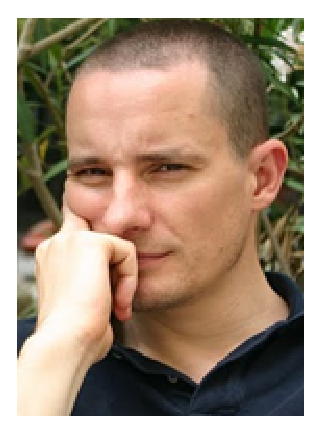
\includegraphics[width=19mm]{mikolaj}
\end{minipage}
\begin{minipage}[b]{0.4\linewidth}
\centering
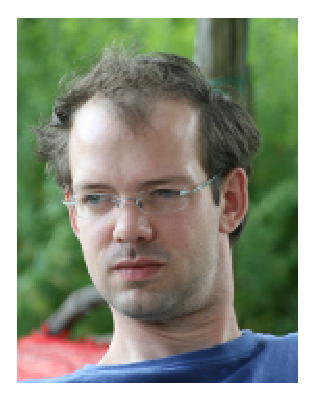
\includegraphics[width=20mm]{thomas}
\end{minipage}
\end{figure}
\end{frame}

\begin{frame}{Counter-example for the general case}
\begin{center}
\begin{figure}
\begin{picture}(65,40)(0,0)
	\rpnode[Nmarks=i,polyangle=45](v_0)(0,30)(4,3){}

	\rpnode[polyangle=45](v_1)(20,40)(4,3){}
	\rpnode[polyangle=45](v_2)(40,40)(4,3){}
	\put(45,39.5){\begin{Huge}$\ldots$\end{Huge}}
	\rpnode[polyangle=45](v_n)(60,40)(4,3){}
	\put(65,39.5){\begin{Huge}$\ldots$\end{Huge}}

	\rpnode[polyangle=45](u_11)(20,12)(4,3){}
	\rpnode[polyangle=45](u_12)(20,0)(4,3){}

	\rpnode[polyangle=45](u_21)(40,24)(4,3){}
	\rpnode[polyangle=45](u_22)(40,12)(4,3){}
	\rpnode[polyangle=45](u_23)(40,0)(4,3){}

	\rpnode[polyangle=45](u_n)(60,12)(4,3){}
	\put(65,11.5){\begin{Huge}$\ldots$\end{Huge}}

	\drawedge(v_0,v_1){}
	\drawedge(v_1,v_2){}
	\drawedge(v_1,u_11){}
	\drawedge(v_2,u_21){}
	\drawedge(v_n,u_n){}

	\drawedge[curvedepth=5](u_11,u_12){$i$}
	\drawedge[curvedepth=5](u_12,u_11){$r$}

	\drawedge[curvedepth=5](u_21,u_23){$i$}
	\drawedge[curvedepth=5](u_23,u_22){$i$}
	\drawedge[curvedepth=5](u_22,u_21){$r$}

	\drawloop[loopdiam=10,loopangle=-90,dash={3 1.5}{1.5}](u_n){$n$}
\end{picture}
\end{figure}
\end{center}

Eve wins but she does not know the bound!

\end{frame}

\subsection{The case of finite graphs}

\begin{frame}{A simple proof for the case of finite graphs}
Condition: parity and all counters are bounded.
\vskip1em

Define:
\begin{itemize}
	\item $\WE(N)$ the set of vertices where Eve wins for the bound $N$.
	\item $\WE$ the set of vertices where Eve wins for some (non-uniform) bound.
\end{itemize}

\pause
\begin{lemma}
\begin{enumerate}
	\item $\WE(0) \subseteq \WE(1) \subseteq \cdots \subseteq \WE(N) \subseteq \WE(N+1) \subseteq \cdots \subseteq \WE$.
\pause
	\item There exists $N$ such that $\WE(N) = \WE(N+1) = \cdots$.
\pause
	\item
For such $N$, Adam wins from $V \setminus \WE(N)$, hence $\WE = \WE(N)$.
\end{enumerate}
\end{lemma}
\end{frame}

\subsection{The case of pushdown graphs}

\begin{frame}{Some more examples (2)}
\begin{figure}
\begin{center}
\begin{picture}(45,25)(0,0)
	\gasset{Nh=6,Nw=6}

	\rpnode[Nmarks=i,iangle=90,polyangle=45](q_0)(0,20)(4,4){}
	\rpnode[polyangle=45](q_1)(20,20)(4,4){}
	\rpnode[polyangle=45](q_2)(20,0)(4,4){}
	\rpnode[polyangle=45](q_3)(40,0)(4,4){}
	\rpnode[polyangle=45](q_4)(45,20)(4,4){}

	\drawloop[loopangle=180](q_0){$\push(a)$}
	\drawloop[loopangle=180](q_2){$\push(b)$}
	\drawloop[loopangle=0](q_3){$\begin{array}{c} \pop(b) \\ i \end{array}$}
	\drawloop[loopangle=0](q_4){}

	\drawedge(q_0,q_1){}
	\drawedge[ELside=r](q_1,q_2){$\pop(a)$}
	\drawedge(q_2,q_3){}
	\drawedge[curvedepth=-5](q_3,q_1){}
	\drawedge(q_1,q_4){}

\only<2>{\node[fillcolor=magenta,Nw=4,Nh=4](pebble)(0,20){}}
\only<3>{\node[fillcolor=magenta,Nw=4,Nh=4](pebble)(20,20){}}
\only<4>{\node[fillcolor=magenta,Nw=4,Nh=4](pebble)(20,0){}}
\only<5>{\node[fillcolor=magenta,Nw=4,Nh=4](pebble)(40,0){}}
\only<6>{\node[fillcolor=magenta,Nw=4,Nh=4](pebble)(20,20){}}
\only<7>{\node[fillcolor=magenta,Nw=4,Nh=4](pebble)(45,20){}}
\end{picture}
\end{center}
\end{figure}
\vskip1em
Adam may use the stack as ``credit''.
\end{frame}

\begin{frame}{Proof sketch}
Condition: parity and all counters are bounded.
\vskip1em

Define:
\begin{itemize}
	\item $\WE(N)$ the set of vertices where Eve wins for the bound $N$ \textbf{in the limit}.
	\item $\WE$ the set of vertices where Eve wins for some (non-uniform) bound.
\end{itemize}

\pause
\begin{proposition}
\begin{enumerate}
	\item $\WE(0) \subseteq \WE(1) \subseteq \cdots \subseteq \WE(N) \subseteq \WE(N+1) \subseteq \cdots \subseteq \WE$.
	\item There exists $N$ such that $\WE(N) = \WE(N+1) = \cdots$.
	\item For such $N$, Adam wins from $V \setminus \WE(N)$, hence $\WE = \WE(N)$.
\end{enumerate}
\end{proposition}
Why is 2. true?
\end{frame}

\begin{frame}{Regularity of the winning regions}

\begin{center}
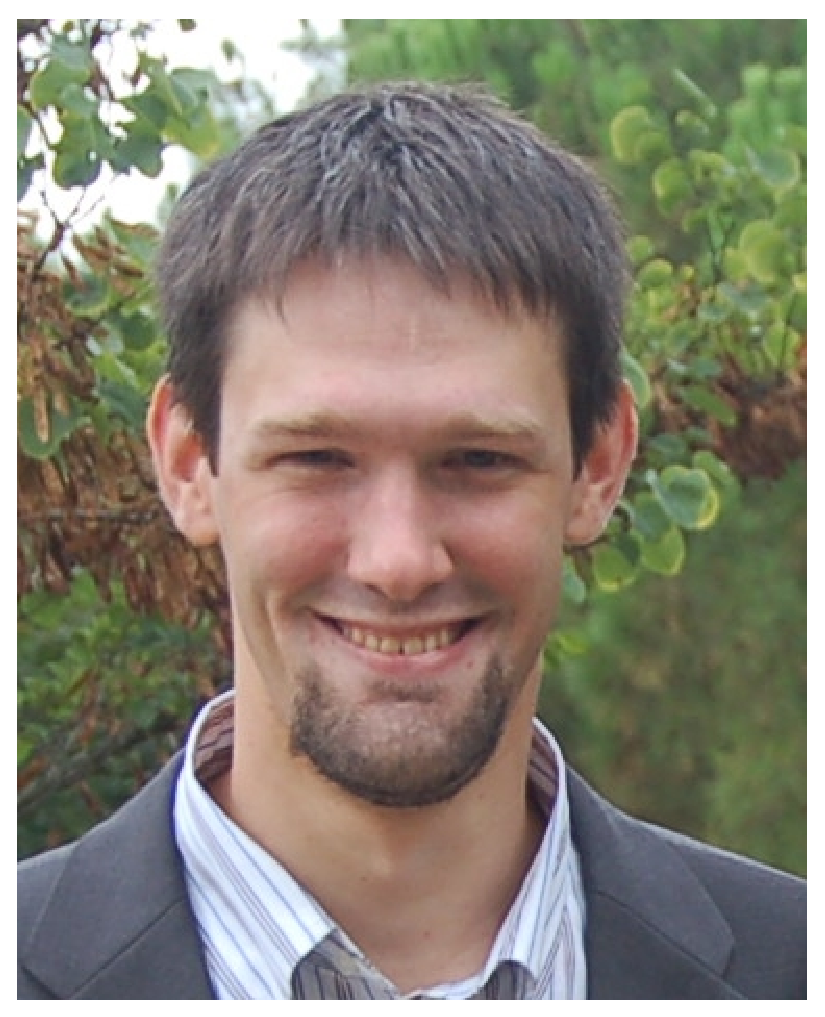
\includegraphics[width=20mm]{serre}
\end{center}

\begin{theorem}[derived from Serre]
For all $N$, $\WE(N)$ is a regular set of configurations, recognized by an alternating automaton
of size $|Q|$ (\textbf{independent of} $N$).
\end{theorem}
\end{frame}

\begin{frame}{Decidability}

\begin{theorem}
For all pushdown games, the following are equivalent:
\begin{itemize}
	\item $\exists \sigma$ (strategy for Eve), $\forall \pi$ (paths), $\exists N \in \mathbb{N}$,\\
$\pi$ satisfies parity and each counter is bounded by $N$.
	\item $\exists \sigma$ (strategy for Eve), $\exists N \in \mathbb{N}$, $\forall \pi$ (paths),\\
$\pi$ satisfies parity and \textbf{eventually} each counter is bounded by $N$.
\end{itemize}
\end{theorem}

\pause
\begin{corollary}
Determining the winner in a pushdown $\omega B$-game is decidable.
\end{corollary}

\pause
Remark: one can show that the collapse bound is doubly-exponential!
\end{frame}

\subsection{Application: $\omega B$-games with max}

\begin{frame}{The max operator}
We add a new feature for counters: $\gamma \leftarrow \max(\gamma_1,\gamma_2)$.

\begin{theorem}[derived from Boja{\'n}czyk and Toru{\'n}czyk]
Deterministic max-automata are equivalent to Weak MSO + $\mathbb{U}$.
\end{theorem}

\vskip1em
We consider $\omega B$-games with max.
\end{frame}

\begin{frame}{Co-determinisation}
\begin{figure}
\begin{center}
\begin{picture}(100,40)(0,0)
	\gasset{Nw=5,Nh=5,Nframe=n}

  	\node(11)(0,30){$0$}
  	\node(12)(15,30){$1$}
  	\node(13)(30,30){$0$}
  	\node(14)(55,30){$0$}
  	\node(15)(80,30){$2$}
  	\node(16)(105,30){$3$}

  	\node(21)(0,15){$0$}
  	\node(22)(15,15){$0$}
  	\node(23)(30,15){$1$}
  	\node(24)(55,15){$2$}
  	\node(25)(80,15){$3$}
  	\node(26)(105,15){$0$}

  	\node(31)(0,0){$0$}
  	\node(32)(15,0){$1$}
  	\node(33)(30,0){$2$}
  	\node(34)(55,0){$3$}
  	\node(35)(80,0){$0$}
  	\node(36)(105,0){$3$}
  	
  	\drawedge(11,12){$i$}
  	\drawedge(12,13){$r$}
  	\drawedge(13,14){}
  	\drawedge(14,15){$\max(\gamma_1,\gamma_2)$}
  	\drawedge(15,16){$i$}

  	\drawedge(21,22){}
  	\drawedge(22,23){$i$}
  	\drawedge(23,24){$\max(\gamma_2,\gamma_3)$}
  	\drawedge(25,26){$r$}

  	\drawedge(33,34){$i$}
  	\drawedge(34,35){$r$}
  	\drawedge[ELside=r](35,36){$\max(\gamma_1,\gamma_2)$}

	\drawedge[dash={3 1.5}{1.5}](24,15){}

\only<1>{
  	\drawedge(31,32){$i$}
  	\drawedge(32,33){$i$}
	\drawedge[dash={3 1.5}{1.5}](33,24){}
  	\drawedge(24,25){$i$}
	\drawedge[dash={3 1.5}{1.5}](25,36){}
	}
	
\only<2>{
  	\drawedge[linewidth=.6,linecolor=red](31,32){$i$}
  	\drawedge[linewidth=.6,linecolor=red](32,33){$i$}
	\drawedge[linewidth=.6,linecolor=red](33,24){}
  	\drawedge[linewidth=.6,linecolor=red](24,25){$i$}
	\drawedge[linewidth=.6,linecolor=red](25,36){}	
	}
\end{picture}
\end{center}
\end{figure}
\pause
\vskip1em
To prove that a counter value is high, one can count backwards!
\end{frame}

\begin{frame}{Reduction}
We reduce $\omega B$-games with max to pushdown $\omega B$-games (without max).
\pause
\vskip1em
Idea: simulate the game and store the play in the stack.

\vskip1em
Whenever he wants, Adam can declare ``this counter has a very large value'':
from there, play backwards using the stack until a reset is met.
\pause

\begin{theorem}
Determining the winner in an $\omega B$-game with max is decidable.
\end{theorem}
\end{frame}

\begin{frame}{The end.}
\addtocounter{framenumber}{-1}
Thank you!
\end{frame}

\begin{frame}{Outline}
\addtocounter{framenumber}{-1}
\tableofcontents
\end{frame}

\end{document}

